\documentclass{article}

\usepackage{fullpage}
\usepackage{amsfonts, amsmath}
\usepackage{url}
\usepackage{hyperref}
\usepackage{graphicx}
\usepackage[final]{pdfpages}

\pagenumbering{gobble}

\hypersetup{
    colorlinks=true,
    linkcolor=black
}

\begin{document}
\clearpage
\vspace*{\stretch{2}}
\begin{center}
\begin{minipage}{.6\textwidth}

\title{Automatic Music Generator \\ \vspace{2 pt} \Large{Project Proposal}}
\author{Sam Fleckenstein (sef44)\\*Ross Nanopoulos (rdn21)}
\date{February 7, 2014}
\maketitle

\end{minipage}
\end{center}
\vspace{\stretch{3}}
\clearpage

\tableofcontents
\newpage

\section{Abstract}
The purpose of this project is to develop an intelligent music composer that will analyze common and popular patterns in music, reason about those patterns, and generate a new piece of music that is significantly different than the analyzed pieces, while still being interesting.

\section{Background}
What is the process by which humans make music? They study the fundamentals: beats, measures, time and key signatures, tempo, rhythm. They listen to great composers: Bach, Tchaichovsky, Mahler, Debussy, Chopin. Somehow this knowledge combined with creativity yields additional, masterful compositions. How then, does one enable a computer to exhibit this thoughtful creativity?\\
\\
A variety of methods have been proposed for algorithmic compositon including hidden markov models, genetic algorithms, neural networks, or a combination thereof. Additionally, a field known as "combination theory" has combined these methods to create more advanced learning and composition algorithms. Neural networks are best suited for learning note by note progressions, but not so well suited for learning an entire musical form. This is due to neural networks examining the local data, but not the entire set of data as a whole. Genetic algorithms involve "mutating" compositions by swapping notes, groups of notes, pitches, etc. These new children compositions, however, can become extremely similar to their parent compositions. Hidden Markov Models utilize an element of probability and uncertainty that can lead to much more interesting compositions, which is the primary method of algorithmic composition that the system in this report will use. Please see the references for more information about these different algorithms.

\section{Intended Audience}
Researchers who would like to incorporate different learning techniques for algorithmic composition will be able to easily integrate with this system. Additionally, anyone who would like to compose music without any talent for a musical instrument.

\section{Software Specifications}
\subsection{UI}
\begin{enumerate}
\item The UI will prompt the user for a musical genre
\item The UI will prompt the user for a song tempo
\item The UI will prompt the user for a time signature
\item The UI will prompt the user for a key signature
\end{enumerate}

\subsection{Echo Nest Interface}


\subsection{Learning Agent}


\subsection{Composition Agent}


\subsection{User Feedback}


\section{Requirements}
\subsection{Song Parser}
The backbone of the song parser will be The Echo Nest's large database of music intelligence. The song parser will utilize The Echo Nest's API to extract useful song information from the database, which includes a plethora of aspects including time signature, key, mode, tempo, loudness, duration, end of fade in, start of fade out, audio fingerprints, timbre, pitch, and loudness. Additionally, The Echo Nest provies sequenced data as "musically relevant elements" that include segments, tatums, beats, bars, and sections. This information will allow the learning agent to discern the myriad dynamics of songs and learn about the ways in which different songs are composed.

\subsection{Learning Agent}
The job of the learning agent will be to take the raw music data gathered by Echo Nest and discover the relevant patterns in the music. There are a number of different algorithms that could be used to achieve this goal, but this project use a hidden Markov model to extract these patterns. This model was chosen because it can be used to represent processes where not all of the information about a state is known. This is useful because music is very complex and it is very difficult to determine every variable that goes into determining what should come next in a song. Another reason that hidden Markov models were chosen for this project is because they have been successfully applied the automatic generation of music.\\
\\
The learning agent is to be designed and implemented in such a way as to allow it to be easily swapped out for a different algorithm. This has several benefits. First, it will be easy to implement a completely different learning algorithm if one does not produce high enough quality results. Second, this will allow for easier testing of the various components of the project. It will be easy to set up dummy functions in the learning agent to accept data from the song parser in order to verify that the parsing is happening correctly. Dummy functions can also be used to pass specific patterns to the composition agent in order to verify that the patterns are applied correctly.

\subsection{Composition Agent}
The composition agent will take the information that the learning agent provides and decide which notes, patterns, rhthyms, etc. to incoproate into its own piece of music. It will then be responsible for outputting this generated music to a .wav file, which can be used later for further analysis.

\section{Project Management}
Below is a Gantt Chart, which will drive our development process and schedule:
\begin{figure}[ht]
\center{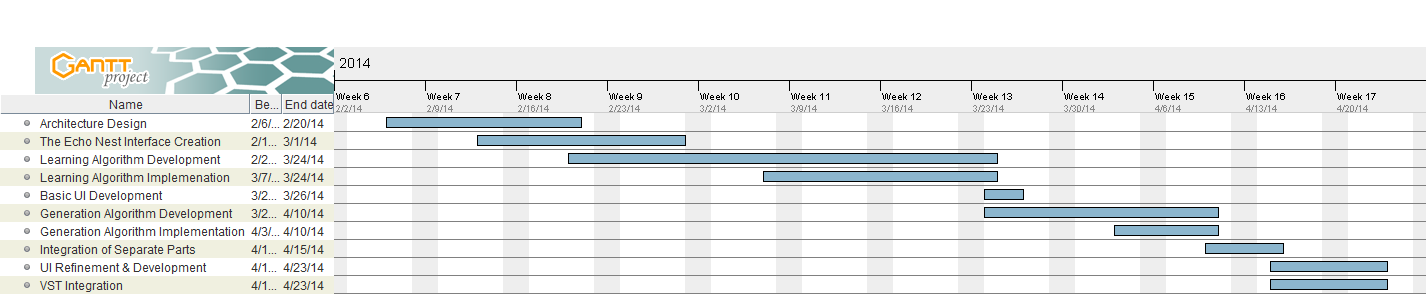
\includegraphics[width=\linewidth]{gantt.png}}
\end{figure}

\subsection{Communication}
In order to facilitate on-time delivery of the Intelligent Music Generator, in-person meetings will be held at least once at week on Thursdays at 4:30. In addition to this, meetings will be held as necessary to discuss upcoming deadlines as well as any issues that have come up. Communication will also happen during the rest of the week primarily via email.

\subsection{Source Control}
Github will be used for feature tracking and reporting bugs.  Pull requests will be utilized to ensure that each member has reviewed the code before it enters the master branch.  Branches will be utilized for implementing different components and features.

\subsection{Work Division}
The primary responsibilities of each of the project members are as follows. Sam will be responsible for the primary development and implementation of the learning algorithms. Ross will be in charge of the implementation of the rest of the project. This is not a hard division of the work as each of the group members will also be working a great deal on the parts of the project they are not in charge of. This division of work fits well with the strengths and experience of each of the project members.

\section{Completed Work}
The work that is completed so far has been mostly research based. Various learning techniques for the learning agent have been examined before settling on using a Hidden Markov model. This model was chosen for several reasons. First, because it has been applied to various other projects with similar goals to this one. Second, because it appears to be complex enough to produce interesting music, but simple enough that it will be possible to complete the project in the given timeline.\\
\\
Pseudo-code has been written for the learning agent in order to more fully understand what will be required to implement the agent.  Additionally, preliminary components of the parser have been designed and implemented; however, it currently only makes a call to the The Echo Nest's API with limited parameters.

\section{Wishlist Features}
There are a number of features that will be included in the project if the required components are completed in time. First is some sort of user friendly UI. Currently, the only planned way of interacting with the program is through the command line. Since this method is not particularly user friendly, a UI with user controls may be added.\\
\\
Another feature that may be added is a different learning algorithm. If there is time, neural networks or genetic algorithms may be explored and added to do the learning, instead of just using a hidden Markov model.\\
\\
A third feature that will be added if there is time is the ability to output the music to a Virtual Studio Technology. This would allow songs to be created that have more than one instrument. It would also allow the user or program to select what instrument they would like to use.

\section{Software Requirements}
\subsection{Song Parser}
The song parser will contain the interface for interacting with The Echo Nest's API and database. It will make a call using the API determined by user input. It will be fed a seed note, chord, key, or other attributes from which the parser can locate and return relevant songs. For example, the song parser could be passed in a genre of rock, with a seed note of "A", a time signature of 4/4, and a tempo of 180-200 beats per minute. This will allow the calls to The Echo Nest's API to be more specific, so that the other parts of the automatic music generator will have more specific data with which to reason. The Echo Nest's API returns JSON objects that can be passed on by the song parser, in order to be used by the learning agent in its reasoning.

\subsection{Learning Agent}
\subsubsection{Internal Architecture}
The learning agent will have two main components. The first part will be the algorithm responsible for extracting patterns from the music. It will work by constructing a model of how it perceives a model of the music to be structured. This includes a representation of the observed outputs (pitches, note durations, chord progressions, key changes, etc) of the hidden states of the musical model. After receiving these outputs from the song parser, this algorithm will find the most useful and interesting patterns and output them.\\
\\
In order for the learning algorithm to work properly, it needs to be provided with estimated values of the hidden parameters in the music (i.e. the probabilities of transitioning between the hidden states). These values will come from a second algorithm, namely the Baum-Welch algorithm, which works by finding the maximum likelihood estimate of the hidden parameters, given the observed data. That is, it finds the values for the transition parameters that make the observed data most likely. 

\subsubsection{Parser to Learning Agent Interface}
In order to make the learning agent as modular as possible, the interface between it and the song parser will be kept very small, and will consist of a single call to the parser to get the raw song data. This will make it easier to swap out the learning algorithm if the need arises.

\subsubsection{Learning Agent to Composition Agent Interface}
Similar to the interface between the parser and the learning agent, this interface between the learning agent and the composition agent will be kept as small as possible. The only interaction between these two components will be when the learning agent passes the composition agent a file containing a representation of all of the relevant patterns that it found in the music.

\subsection{Composition Agent}
The composition agent will take the relevant patterns provided by the learning agent and decide which patterns should be utilized in its composition. It will consist of an algorithm to decide which of the relevant patterns will be chosen, as well as a component to write a .wav file to disk.  Additionally, there will be a component to compare the new song with the songs that were used to create it.

\nocite{*}

\bibliography{References}
\bibliographystyle{plain}

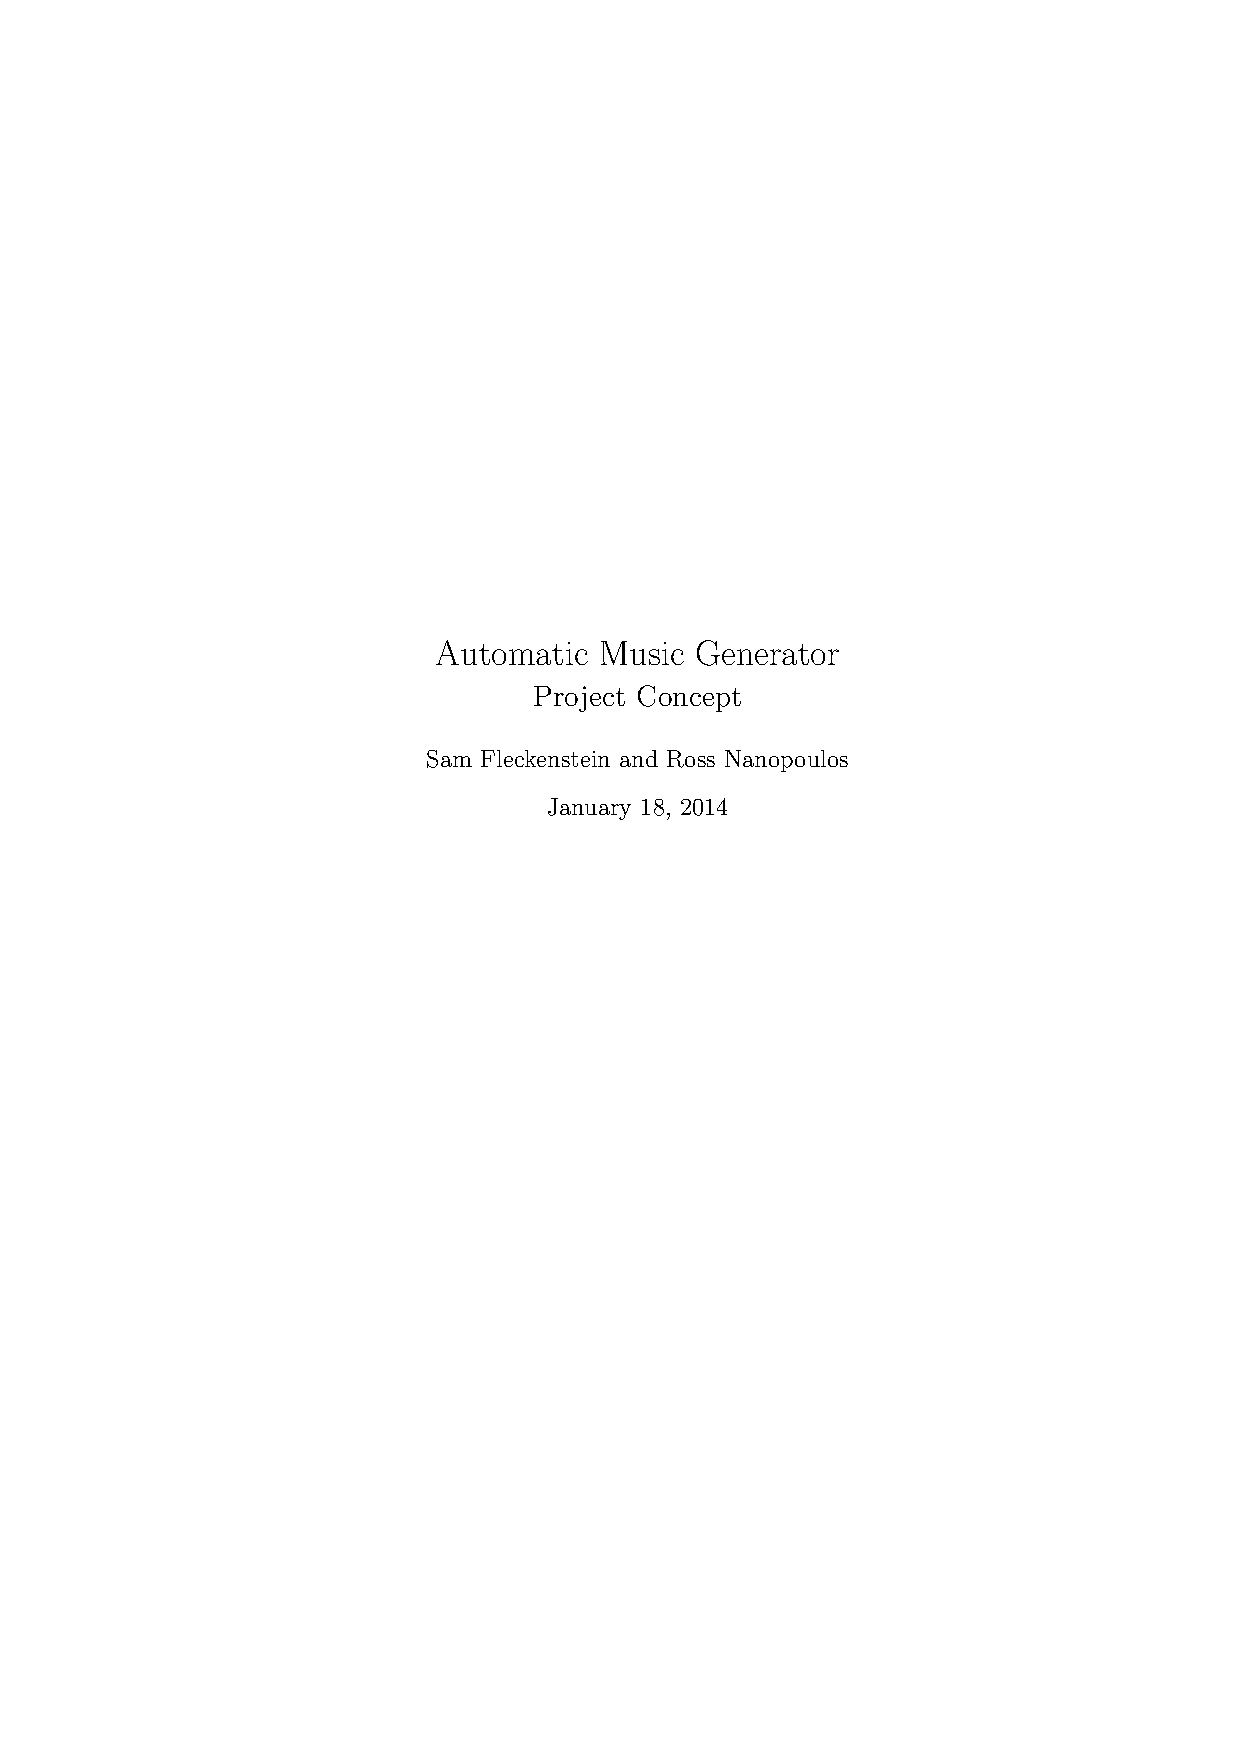
\includepdf[pages=-]{Concept.pdf}

\end{document}
